\section{Introduction}

This work focuses on \qt{shared memory} systems that provide a read/write interface to the programmer. Such systems are ubiquitous in both computer architecture and  distributed systems. Prominent examples include shared memory multiprocessors (SMPs), GPUs, NoSQL Databases~\cite{twitter:2016}, coordination services\cite{Hunt:2010}, and software-based DSMs~\cite{Keleher:1994}.

Such systems commonly replicate data -- sometimes for performance (through caching), sometimes for fault tolerance and sometimes for both.
To enable reasoning in the presence of replication, a \emph{memory consistency model} (\emph{\mcm}) is specified as part of the system's interface, providing the rules that dictate what values a read can return.
In order to enforce the \mcm, the system deploys a protocol which ensures that the replicas behave in accordance to the \mcm. This protocol is called \emph{coherence protocol} in computer architecture and \emph{replication protocol} in distributed systems. We simply refer to it as \emph{the protocol}.

The \mcm\ specifies the behaviour of the system when executing parallel programs by enumerating all patterns through which parallel programs can synchronize.
For example, an \mcm\  $CM_a$ can guarantee the synchronization pattern of \figref{fig:intro-ex}a (commonly known as \qt{producer-consumer}). Specifically, in \figref{fig:intro-ex}a, process P1 writes object $x$ and then $y$, while process P2 reads $y$ and then $x$. 
$CM_a$ guarantees that if P2's read to $y$ returns the write of P1, then P2's read to $x$ will also return the write of P1 (\ie $x=1$).


\begin{figure}[t]
  \centering
  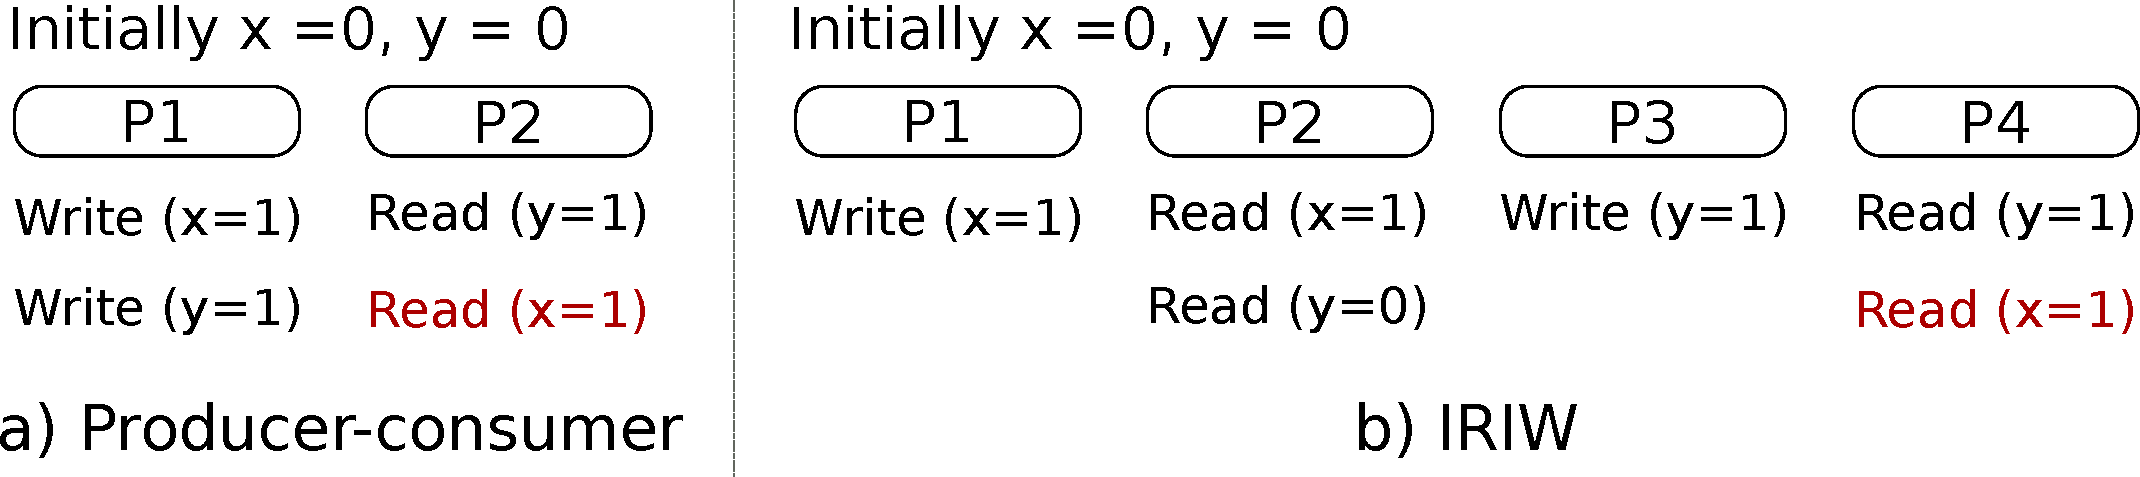
\includegraphics[width=0.48\textwidth]{1_figures/intro-example.pdf}
  \caption{a) The producer-consumer synchronization pattern mandates that if P2 reads P1's write to $y$, then it must also read P1's write to $x$. b) The independent-reads independent-writes (IRIW) pattern mandates that if P2 sees P1's writes but not P3's and P4 sees P3's write, then P4 must see P1's write. }
  \label{fig:intro-ex}
\end{figure}
\custvspace
The \mcm\ is thus  a contract between the programmers and the designers. While programmers must understand the behaviour of the system, the designers must understand how to implement that behaviour.
Problematically, enforcing the \mcm\ is very challenging. 
For instance, consider two well known \mcms: TSO~\cite{Owens:2009} and Causal Consistency (CC)~\cite{Petersen:1997}. TSO enforces both \figref{fig:intro-ex}a and b while CC enforces \figref{fig:intro-ex}a but not b.
Given this information, how is the designer to implement a correct and efficient protocol for either \mcm?
Crucially, how is the designer to differentiate between the two models? E.g., how can one exploit that \figref{fig:intro-ex}b need not be enforced in the CC protocol? 

\y{
Our overarching vision is to automate the above task: given a target \mcm\ we envision a software tool that can produce an efficient protocol. 
We argue that to create this tool we need one additional level of abstraction which can act as an intermediary between the \mcm\ and the protocol.
That is: (1) we must be able to automatically translate any \mcm\ to this abstraction; and (2) we must also be able to map the abstraction itself 
into protocol design choices.
In this work, we take a step towards actualizing our vision, by  proposing such an abstraction and, most crucially, presenting the mapping from \mcms\ to this abstraction. 
We also informally relate the abstraction to protocol design choices. 

}

To create this abstraction, we observe that a shared memory system, be it a multiprocessor or a geo-replicated Key-Value Store (KVS), can be abstracted through the model of \figref{fig:intro-mod}, which depicts a set of processes executing a parallel program. 
Each process inserts its memory operations to a structure we call the \emph{reorder buffer (\rob)},  allocating one \rob\ entry per operation.
The \emph{memory system} executes the operations it finds in the \rob\ and writes back the response of each operation in-place in its dedicated entry.

A process models a client of a KVS or a core of a multiprocessor. The \rob\ abstracts the core's load-store queue or a software queue that a KVS must maintain to keep track of incoming requests.
The memory system is modelled as a distributed system comprising a set of \emph{nodes}, where each node contains a controller and a memory.
The nodes model the private caches of the multiprocessor or the geo-replicated memory servers of the KVS. Finally the network of the memory system can be thought of as the Network-on-Chip or as the WAN.

We observe that protocols of real systems enforce various consistency models using two widgets: 1) the \rob\ that allows for the reordering of operations; and 2) the memory system which determines how a read or a write executes, \ie how it propagates to each of the replicas. 
We propose two sets of mathematical rules to abstract protocols, one that can abstract the reorderings of the \rob\ and one that can abstract the propagation rules of the memory system.

\begin{figure}[t]
  \centering
  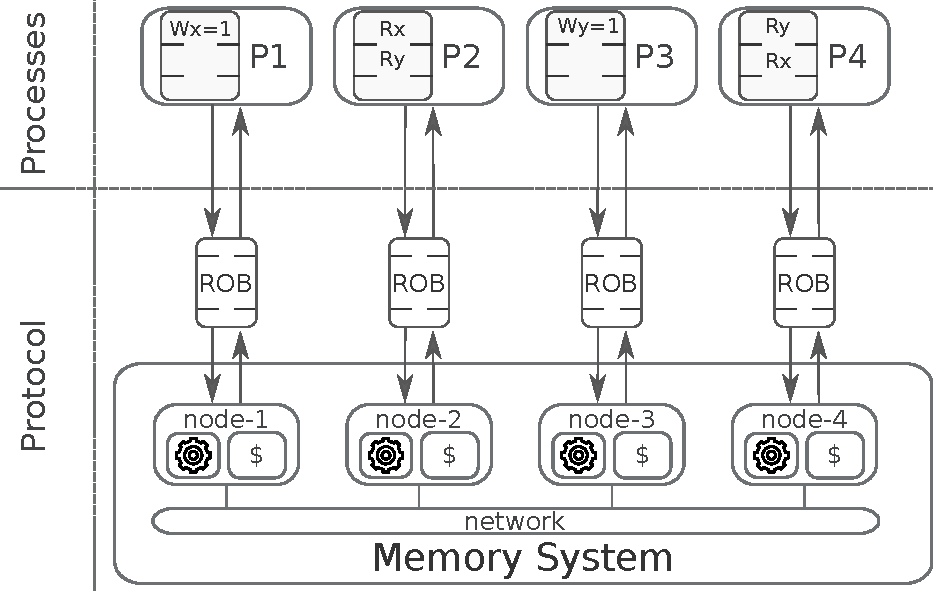
\includegraphics[width=0.45\textwidth]{1_figures/intro-model.pdf}
  \caption{The model of a shared memory system. Processes P1-P4 execute the IRIW pattern of \figref{fig:intro-ex}b. }
  \vspace{-1em}
  \label{fig:intro-mod}
\end{figure}

Specifically, we model the \rob\ using four rules named \emph{program-order real-time orderings} (\emph{\prts}).
The $\prtwr$ \prt\ mandates that when write $w$ precedes read $r$ in a program execution, then $r$ can begin executing in the memory system only after $w$ has completed.
Similarly, we define $\prtww,\prtrr, \prtrw$, for the rest of the combinations between reads and writes.
To summarize, we model an \rob\ by specifying the subset of the four \prts\ it enforces. 

We model the memory system using four rules named \emph{synchronization real-time orderings} (\emph{\srts}).
The $\rtwr$ \srt\ mandates that if write $w$ to object $x$ completes before read $r$ to object $x$ in real time, then $r$ must observe $w$.
Similarly, we define $\rtww, \rtrr, \rtrw$.
To summarize we model a memory system by specifying the subset of the four \srts\ it enforces.

We refer to \prts\ and \srts\ as \emph{real-time orderings} (\emph{\rts}).
The eight \rts\ comprise our designer-centric intermediate abstraction of the protocol. 

\y{
While the \rts\ have been employed by other works in the past to model consistency models or protocols (\S\ref{sec:related}), this work is the first to present a 
mapping from \mcms\ to the \rts. That is, given any \mcm, we provide the set of minimal \rts\ that enforce it. 
Crucially, this mapping, along with relating the \rts\ with protocol implementation techniques, pave the way for automating protocol design.
}

Using this mapping from \mcms\ to \rts, we now revisit the questions we posed on \figref{fig:intro-ex}. Specifically, \prts\ $\prtww$ and $\prtrr$ and the \srt\ $\rtwr$ suffice to enforce the producer-consumer pattern (discussed in \secref{sec:rt-cons:reg-ex}). 
Informally, $\prtww$ mandates that writes from the same process must be executed in the order intended by the program; $\prtrr$ mandates the same for reads; $\rtwr$ mandates that a read must be able to return the value of the latest completed write (from any process).
To also enforce the IRIW pattern, $\rtrr$ is required (discussed in \secref{sec:rt-cons:irreg}). Informally, $\rtrr$ mandates that if a read returns the value of write $w$, then any later read must also be able to return the value of write $w$.

\beginbsec{Contributions}
In summary, in this work we make the following contributions:
\squishlistContrib
\item 
We propose and formalize eight \rts\ for mathematically modelling consistency enforcement protocols, serving as an intermediate abstraction between the \mcm\ and the protocol implementation (\S\ref{sec:rt}).
\item
We create a mapping from \mcms\ to \rts, specifying the minimal set of \rts\ sufficient to enforce any \mcm\ (\S\ref{sec:rt-cons}) \y{and vice versa, specifying the \mcm\ enforced by any set of \rts\ (\S\ref{sec:rt-to-cons})}. 
\item
We informally map \rts\ to protocol implementation techniques (\S\ref{sec:prot}).
\squishend
























